\documentclass[unicode,11pt,a4paper,oneside,numbers=endperiod,openany]{scrartcl}

\renewcommand{\thesubsection}{\arabic{subsection}}

\usepackage{graphicx}
\usepackage{longtable}
\usepackage{booktabs}
\usepackage{multirow}

\usepackage{ifthen}
\usepackage[utf8]{inputenc}
\usepackage{graphics}
\usepackage{graphicx}
\usepackage{hyperref}

\pagestyle{plain}
\voffset -5mm
\oddsidemargin  0mm
\evensidemargin -11mm
\marginparwidth 2cm
\marginparsep 0pt
\topmargin 0mm
\headheight 0pt
\headsep 0pt
\topskip 0pt        
\textheight 255mm
\textwidth 165mm

\newcommand{\duedate} {}
\newcommand{\setduedate}[1]{%
\renewcommand\duedate {\textbf{Due date:}~ #1}}
\newcommand\isassignment {false}
\newcommand{\setassignment}{\renewcommand\isassignment {true}}
\newcommand{\ifassignment}[1]{\ifthenelse{\boolean{\isassignment}}{#1}{}}
\newcommand{\ifnotassignment}[1]{\ifthenelse{\boolean{\isassignment}}{}{#1}}

\newcommand{\punkte}[1]{\hspace{1ex}\emph{\mdseries\hfill(#1~\ifcase#1{Points}\or{Points}\else{Points}\fi)}}


\newcommand\serieheader[6]{
\thispagestyle{empty}%
\begin{flushleft}

\includegraphics[width=0.45\textwidth]{CI_logo}
\end{flushleft}
  \noindent%
  {\large\ignorespaces{\textbf{#1}}\hspace{\fill}\ignorespaces{ \textbf{#2}}}\\ \\%
  {\large\ignorespaces #3 \hspace{\fill}\ignorespaces #4}\\
  \noindent%
  \bigskip
  \hrule\par\bigskip\noindent%
  \bigskip {\ignorespaces {\Large{\textbf{#5}}}
  \hspace{\fill}\ignorespaces \large \ifthenelse{\boolean{\isassignment}}{\duedate}{#6}}
  \hrule\par\bigskip\noindent%  \linebreak
 }

\makeatletter
\def\enumerateMod{\ifnum \@enumdepth >3 \@toodeep\else
      \advance\@enumdepth \@ne
      \edef\@enumctr{enum\romannumeral\the\@enumdepth}\list
      {\csname label\@enumctr\endcsname}{\usecounter
        {\@enumctr}%%%? the following differs from "enumerate"
	\topsep0pt%
	\partopsep0pt%
	\itemsep0pt%
	\def\makelabel##1{\hss\llap{##1}}}\fi}
\let\endenumerateMod =\endlist
\makeatother




\usepackage{textcomp}







\begin{document}


\setassignment
\setduedate{Monday, 19 December 2024, 06:00 PM}

\serieheader{Experimentation and Evaluation}{2024}{\textbf{Students:} Davide Frova, Costanza Rodriguez Gavazzi}{}{Project 2}{}
\newline


\section{Abstract}
This study investigates whether using \texttt{camelCase} or \texttt{kebab-case} as a naming convention affects response time when reading and understanding code identifiers. A total of 36 participants, with and without programming backgrounds, completed timed tasks involving both case styles. Descriptive statistics showed that participants were faster and more consistent with \texttt{camelCase}, especially those without programming experience. Inferential statistics using a paired samples t-test revealed no significant difference between the two styles, suggesting that while \texttt{camelCase} appeared slightly faster, the difference was not statistically significant.

\section{Introduction}
The readability of code is extremely important for developer productivity and collaboration. Part of it, is the style of naming conventions used for identifiers. Two commonly used styles are \texttt{camelCase} (e.g., \texttt{myVariableName}) and \texttt{kebab-case} (e.g., \texttt{my-variable-name}). While every developer has their preference (including us), we wanted to investigate whether one style is more effective than the othe.
In this study, we conducted a controlled experiment to compare response times for tasks involving \texttt{camelCase} and \texttt{kebab-case}. We also comment on descriptive statistics with respect to accuracy, measured as correctness of the answers. Both participants with programming backgrounds were involved.


\subsection{Hypotheses}
\textbf{Null Hypothesis}: There is no significant difference in speed between \texttt{camelCase} and \texttt{kebab-case}. \\
\hfill \\
\textbf{Alternative Hypothesis}: Users perform better with \texttt{kebab-case} compared to \texttt{camelCase}.

\section{Method}

\subsection{Variables}
\subsubsection{Independent Variable} 
\textbf{Case Style}: \texttt{camelCase}, \texttt{kebab-case}

\subsubsection{Dependent Variables}
\textbf{Response Time}: in milliseconds; \\
\textbf{Correctness}: true/false

\subsubsection{Control Variables}
Order of presentation of questions

\subsubsection{Blocking Variable}
\textbf{Previous programming experience}: true/false.

\subsection{Design}
Single-Factor Experiment \\
\hfill \\
Within-Subject Design: Participants experienced both case styles in random order to avoid potential learning effects.
\\
\hfill \\
\begin{figure}[h!]
    \centering
    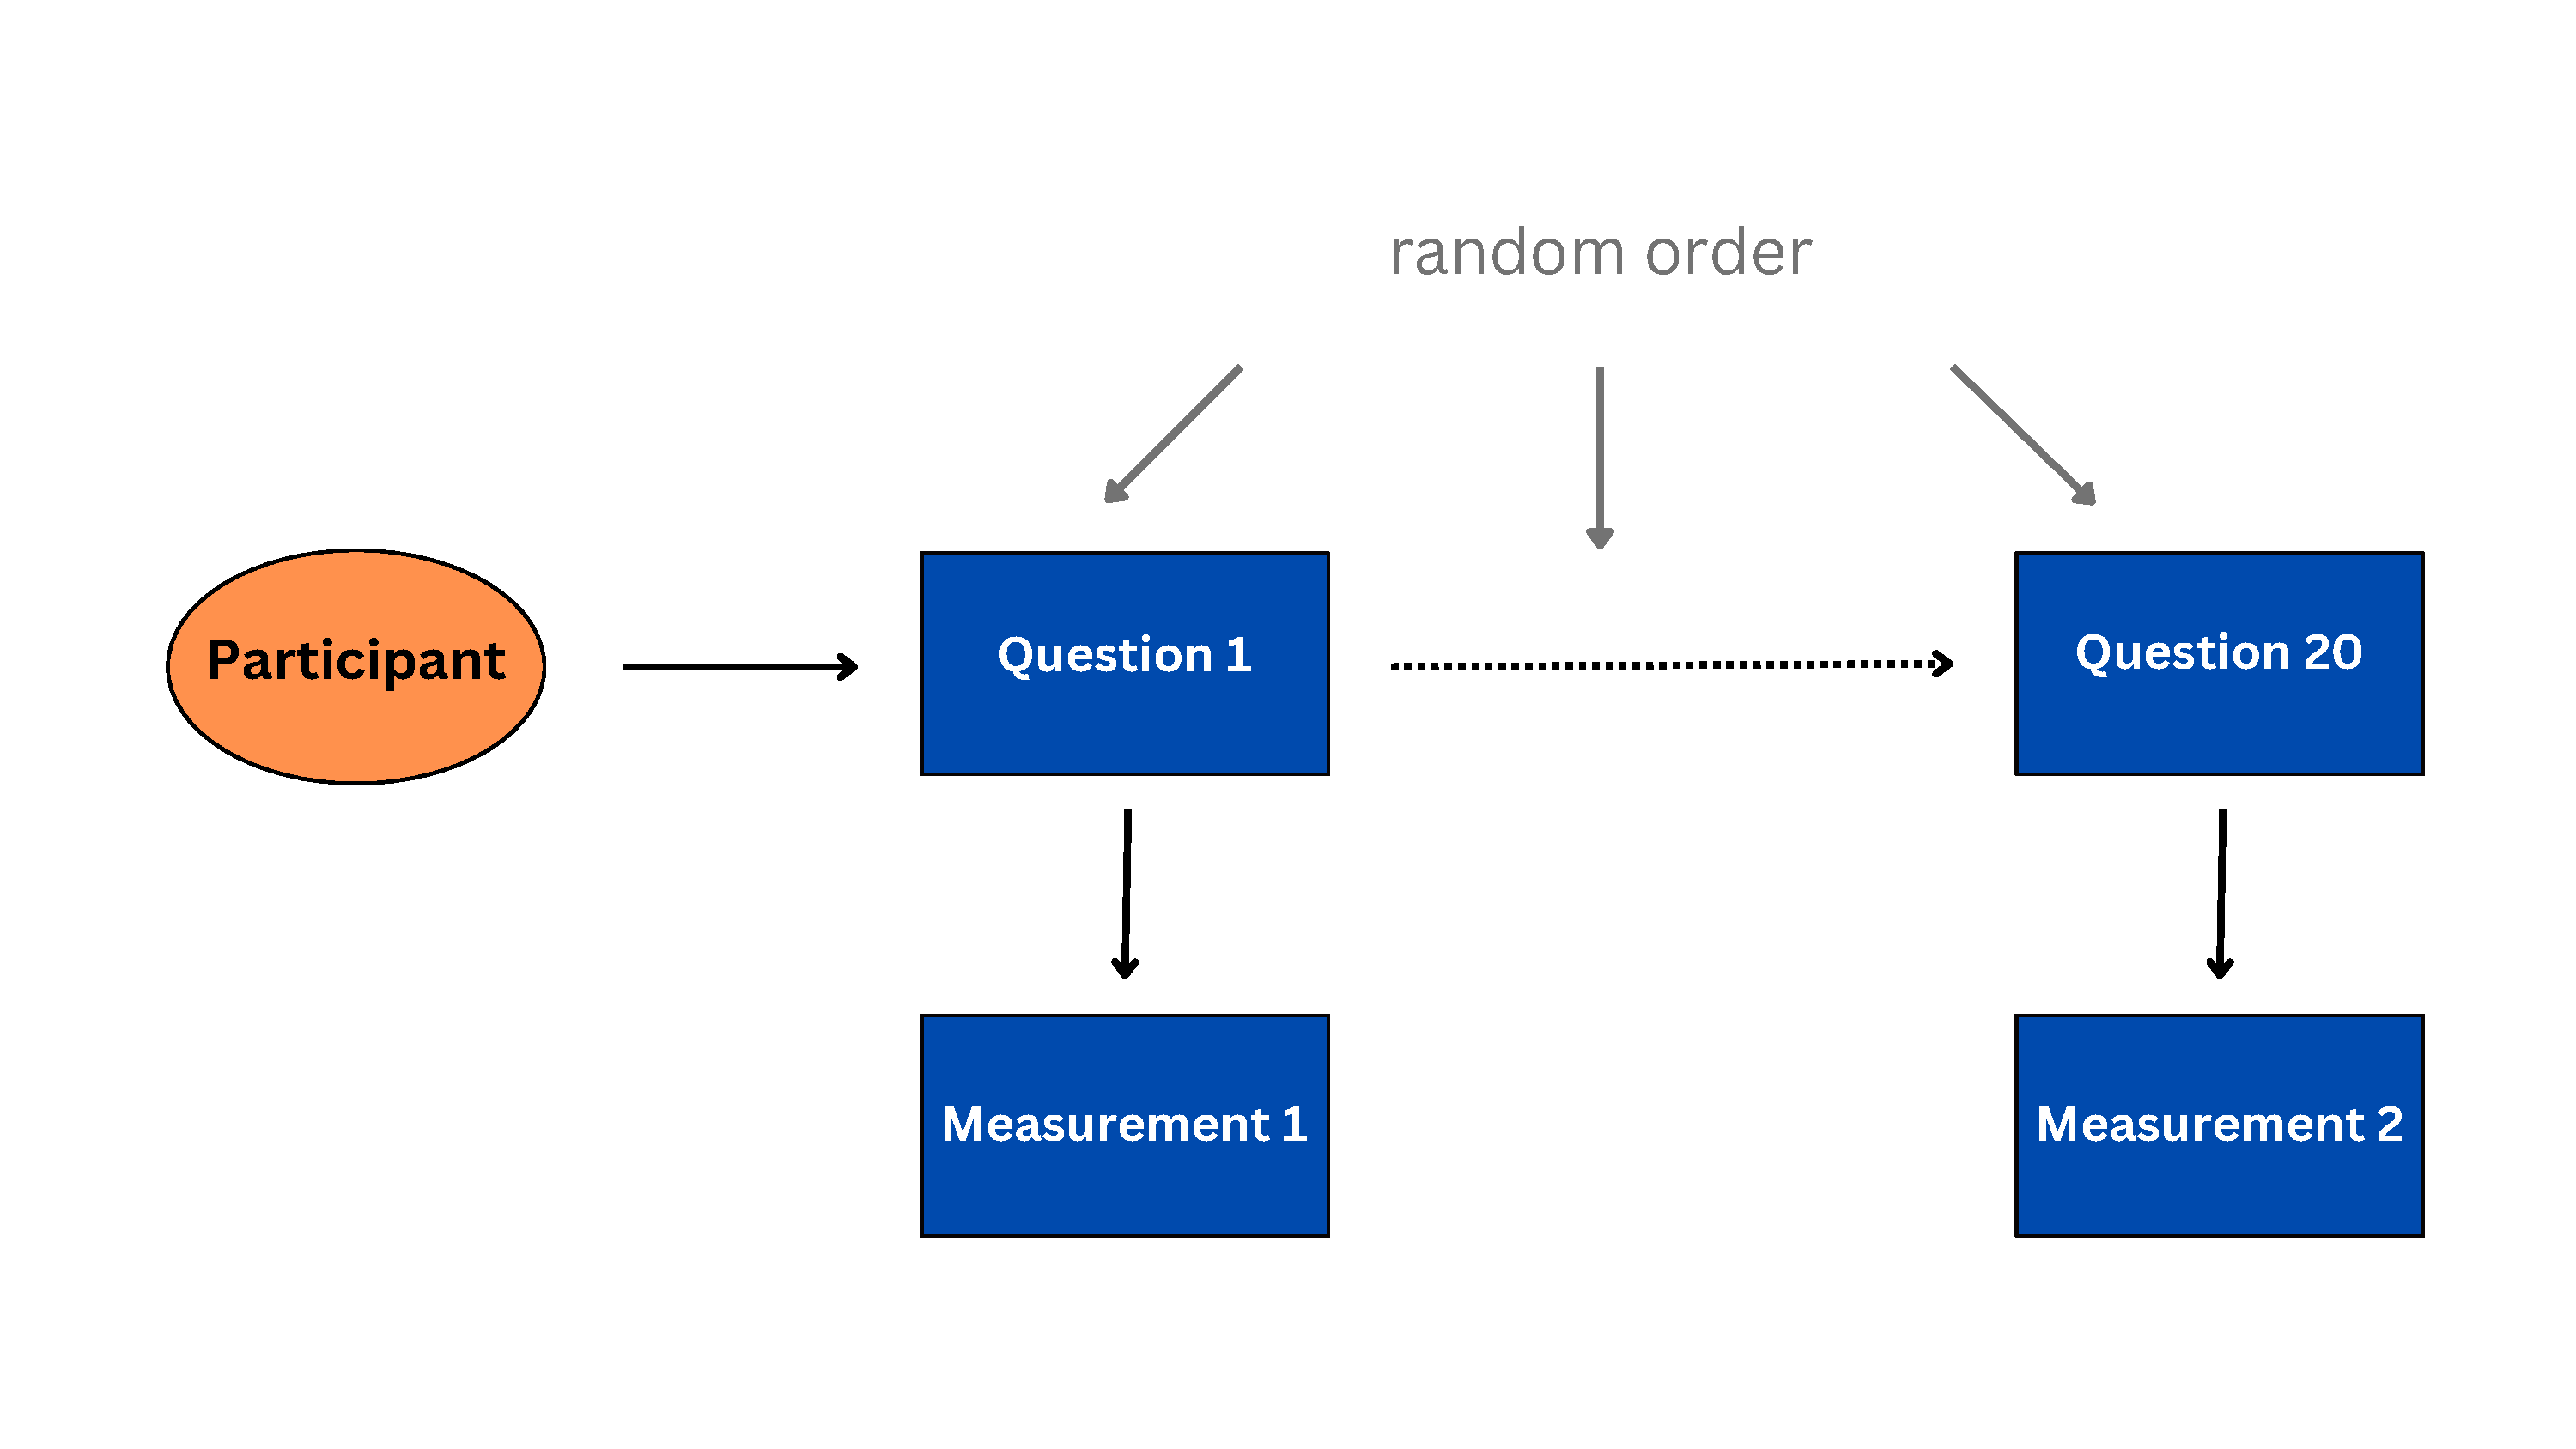
\includegraphics[width=0.7\textwidth]{./figures/graph.pdf}
    \caption{Design of the experiment}
    \label{fig:graph}
\end{figure}

\subsection{Participants}
\textbf{Total participant}: 36 \\
\textbf{Age range}: 20 - 58 \\

\subsection{Apparatus and Materials}
Web app built with Next.js, React, and TypeScript, deployed on Vercel. //todo davide

\subsection{Procedure}
After reading a brief explanation of the experiment participants were asked to:
\begin{itemize}
    \item Provided their age and whether they had programming background.
    \item Completed a warm-up tutorial.
    \item Answer 10 \texttt{camelCase} and 10 \texttt{kebab-case} questions, randomly shuffled.
\end{itemize}

We recorded response times, correctness, age of participant and whether they had a programming background or not.

\section{Results}

\subsection{Visual Overview}

\begin{figure}[h!]
    \centering
    \begin{minipage}{0.45\textwidth}
        \centering
        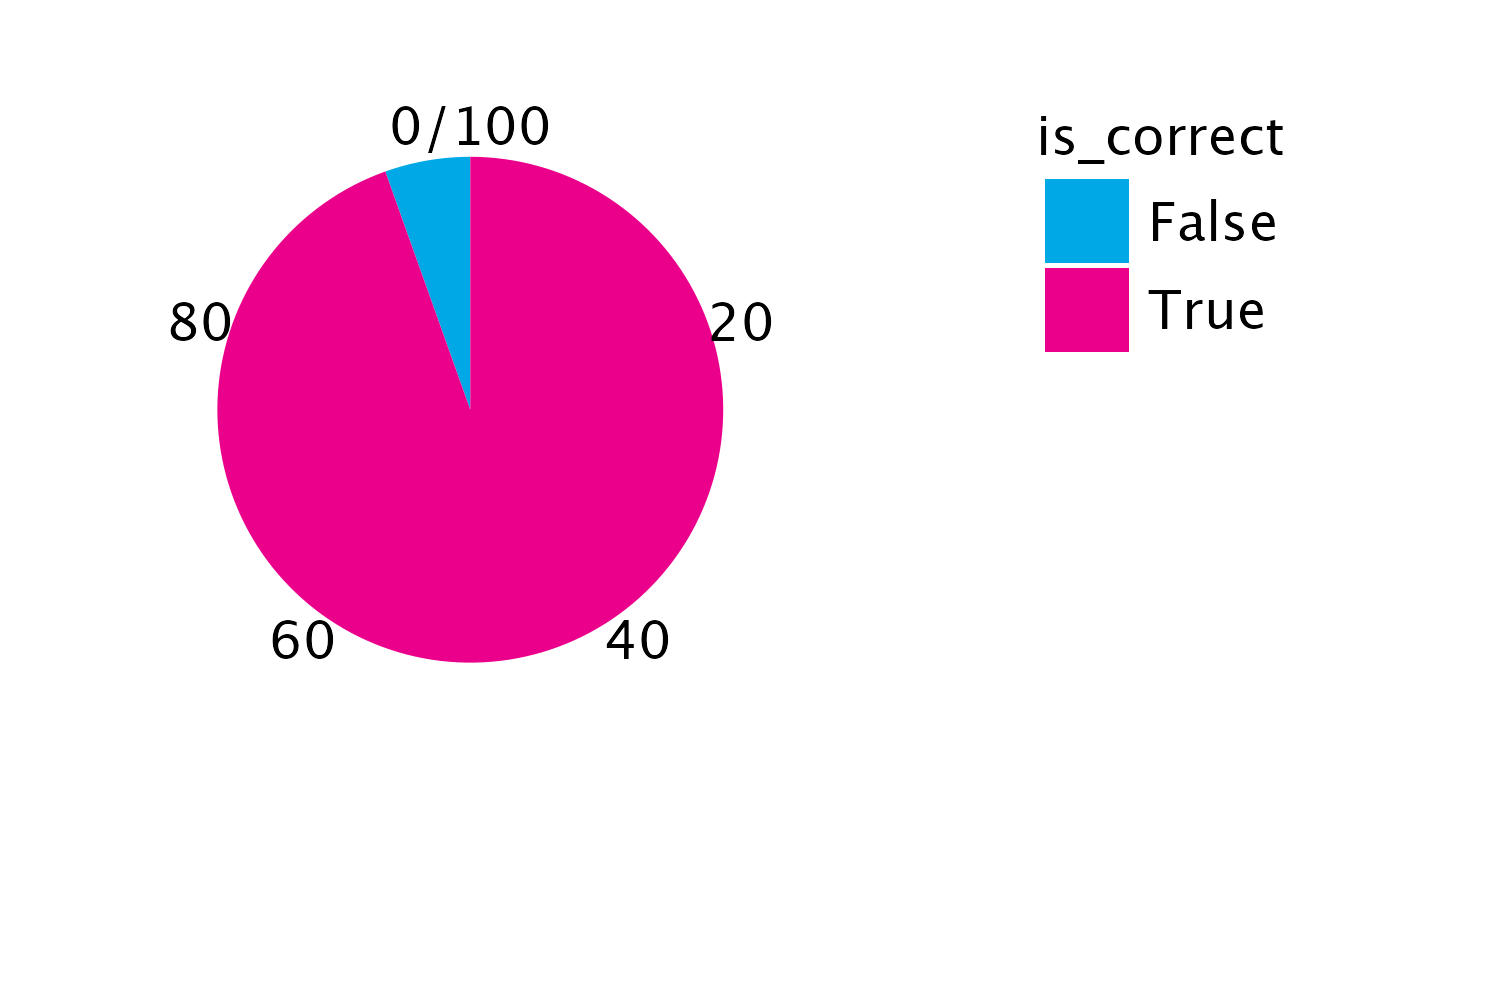
\includegraphics[width=\textwidth]{./figures/correct_camel_noback.png}
        \caption{Correct Answers for \texttt{camelCase} with No Programming Background}
        \label{fig:correct_camel_noback}
    \end{minipage}
    \hfill
    \begin{minipage}{0.45\textwidth}
        \centering
        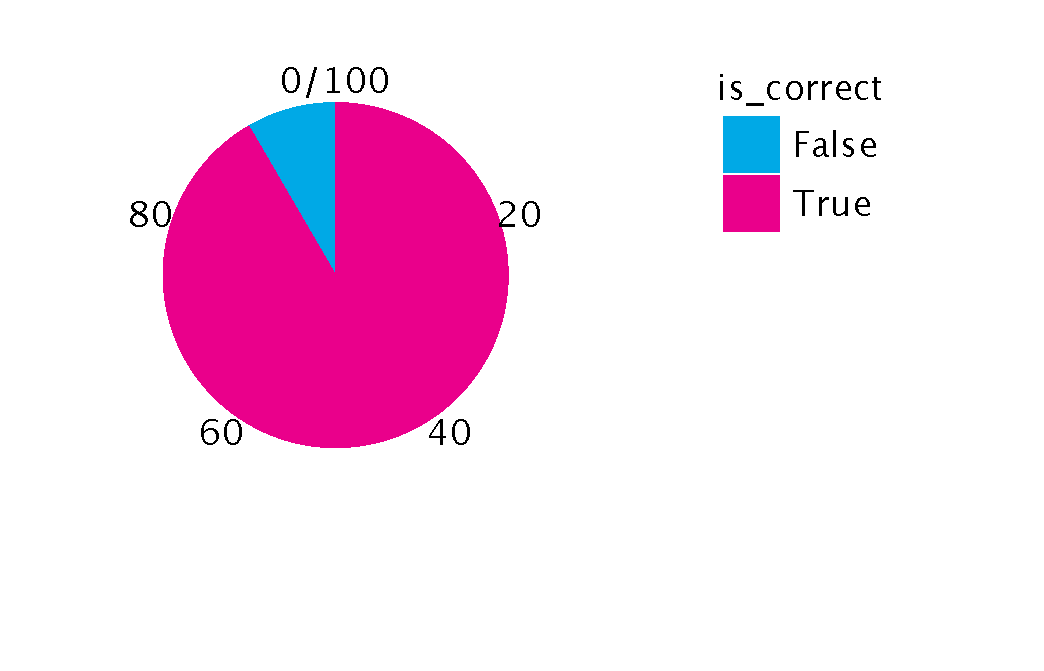
\includegraphics[width=\textwidth]{./figures/correct_camel_background.eps}
        \caption{Correct Answers for \texttt{camelCase} with Programming Background}
        \label{fig:correct_camel_background}
    \end{minipage}
    
    \vspace{0.5cm} 
    
    \begin{minipage}{0.45\textwidth}
        \centering
        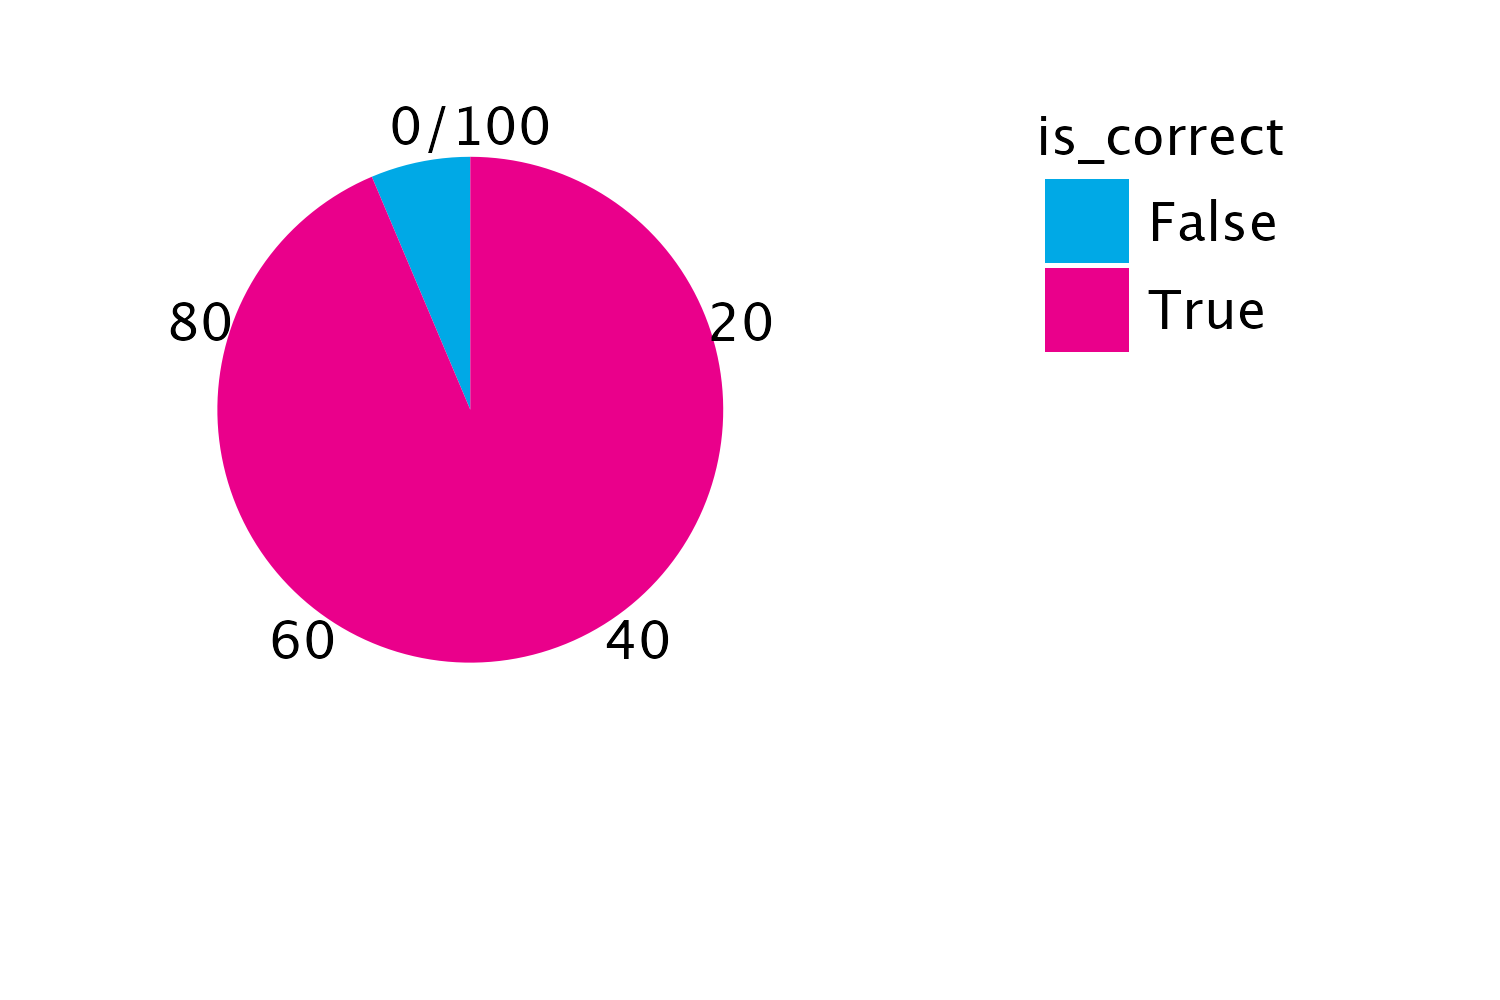
\includegraphics[width=\textwidth]{./figures/correct_kebab_noBack.png}
        \caption{Correct Answers for \texttt{kebab-case} with No Programming Background}
        \label{fig:correct_kebab_noback}
    \end{minipage}
    \hfill
    \begin{minipage}{0.45\textwidth}
        \centering
        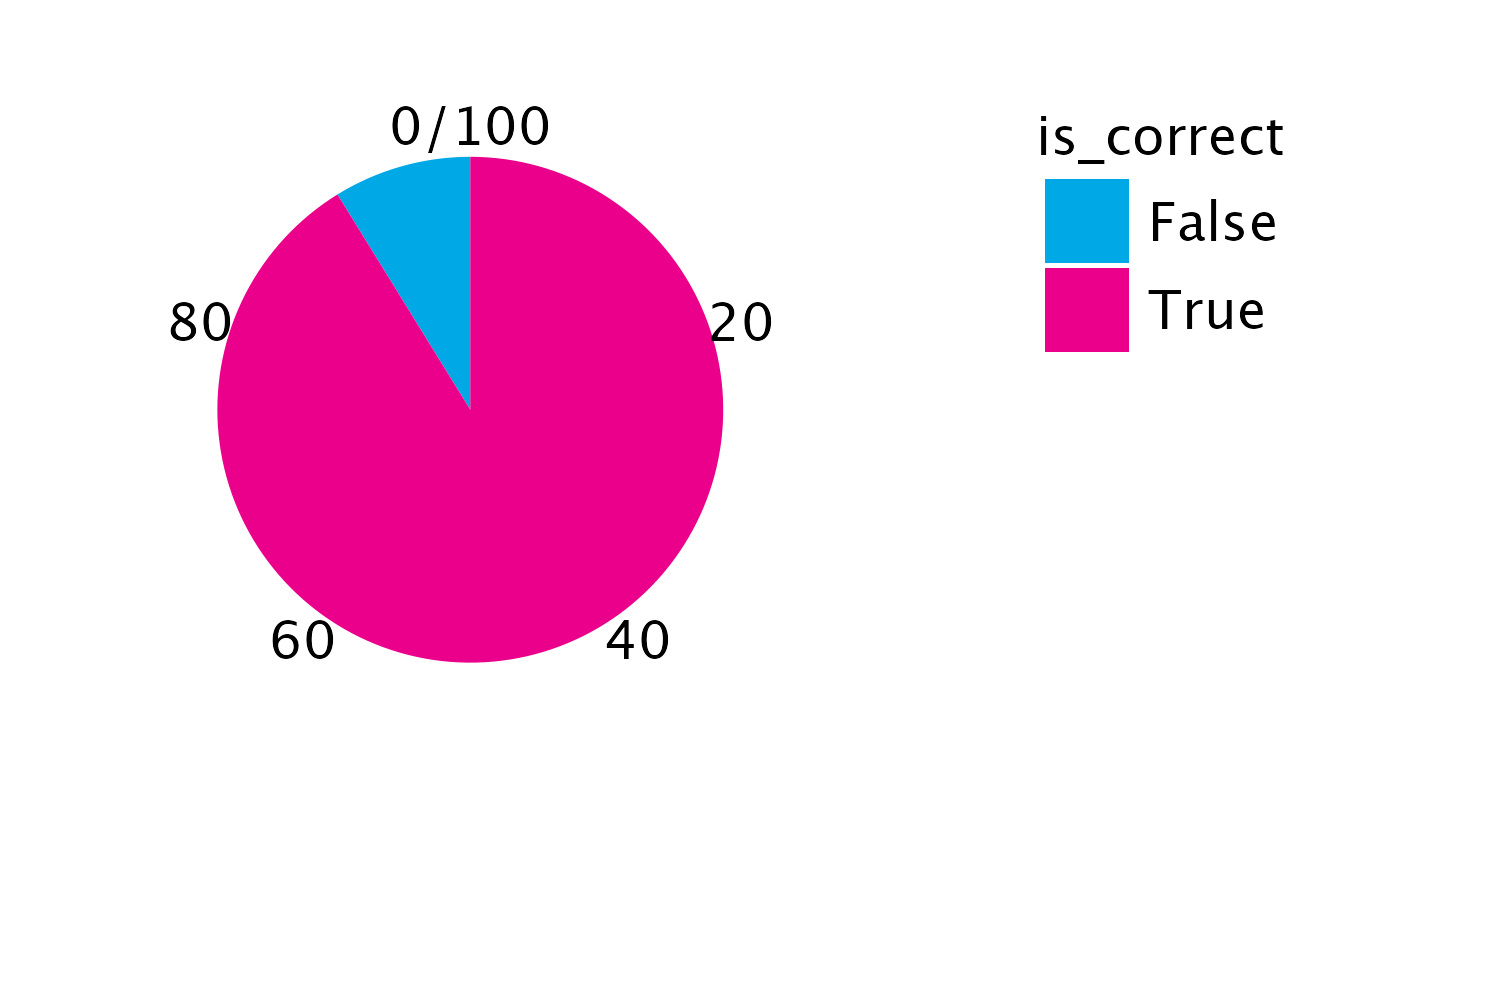
\includegraphics[width=\textwidth]{./figures/correct_keb_backgr.png}
        \caption{Correct Answers for \texttt{kebab-case} with Programming Background}
        \label{fig:correct_kebab_background}
    \end{minipage}
\end{figure}

Looking at how people performed with \texttt{camelCase} in Figure \ref{fig:correct_camel_noback} and Figure \ref{fig:correct_camel_background} and \texttt{kebab-case} in Figure \ref{fig:correct_kebab_noback} and Figure \ref{fig:correct_kebab_background}, we can see that both styles were correct at around 90\%. \\

In particular about 91.4\% of answers were correct in the group of people who had programming experience and 94\% in the group of people who did not have any experience. We hypothesize that the difference in accuracy between the two groups is due to the fact that people with programming experience were quicker to answer - which is later discussed -, and therefore more prone to make mistakes. \\

Figure \ref{fig:boxplot} shows the boxplot of the elapsed time for \texttt{camelCase} and \texttt{kebab-case}. We can see that the median response time (the center line in each box) for \texttt{camelCase} is slightly lower, meaning participants answered faster with this naming style. Furthermore, \texttt{kebab-case} has a wider spread of response times, as we can notice in the number of outliers (dots) above the box.

\begin{figure}[h!]
    \centering
    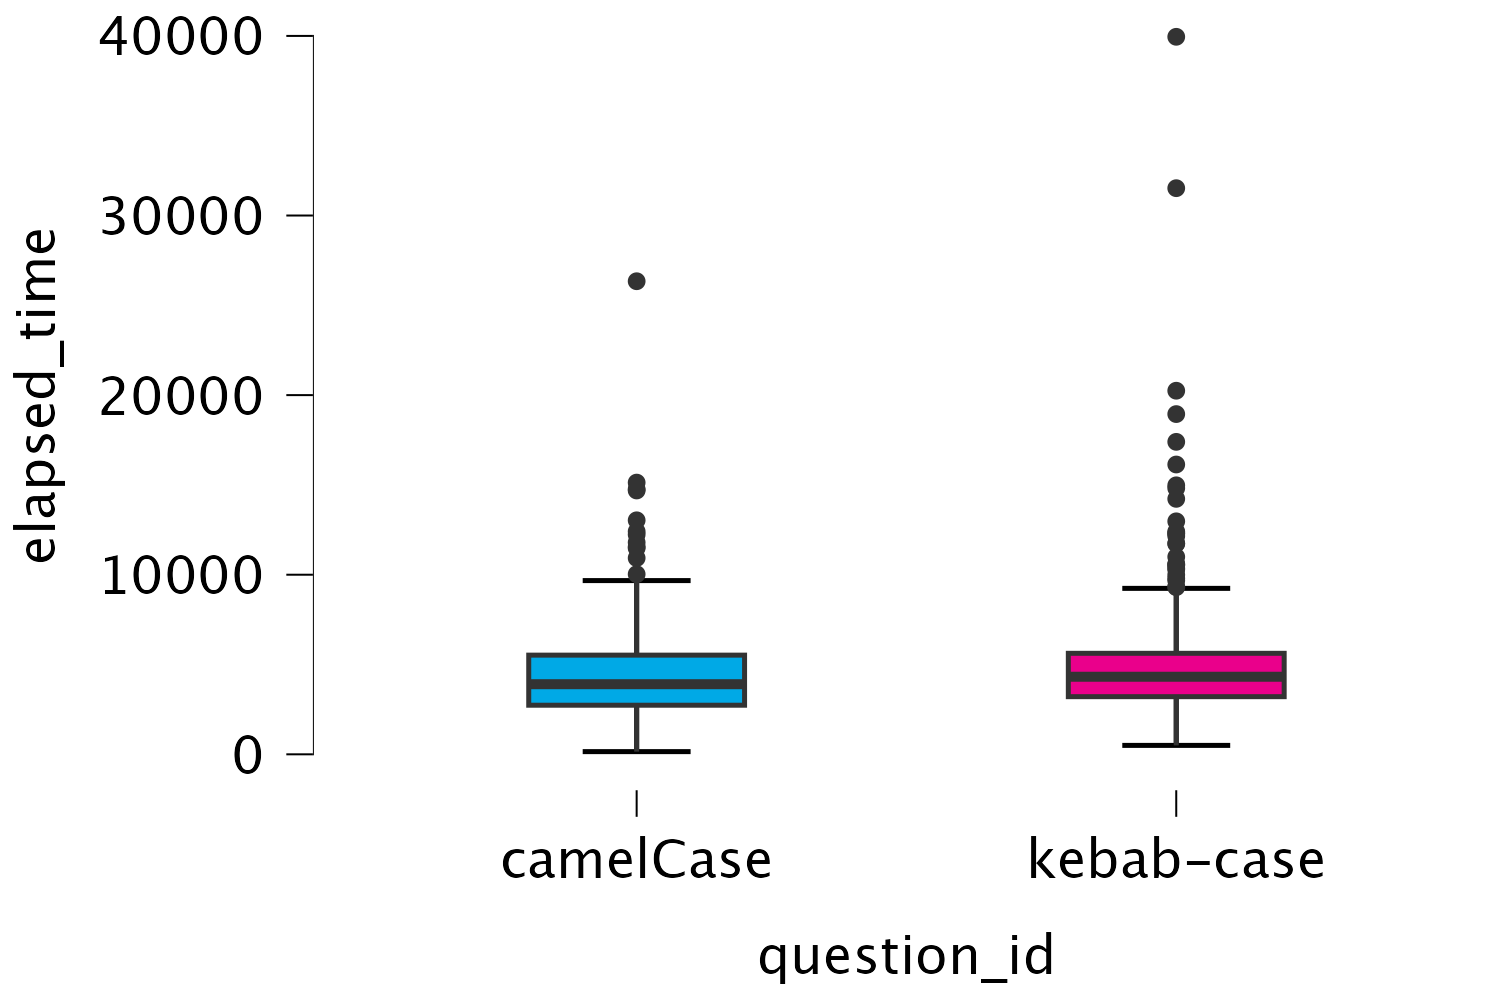
\includegraphics[width=0.7\textwidth]{./figures/elapsed_time_correct.png}
    \caption{\texttt{camelCase} vs \texttt{kebab-case}: Elapsed Time}
    \label{fig:boxplot}
\end{figure}


\begin{figure}[h]
    \centering
    \begin{minipage}{0.45\textwidth}
        \centering
        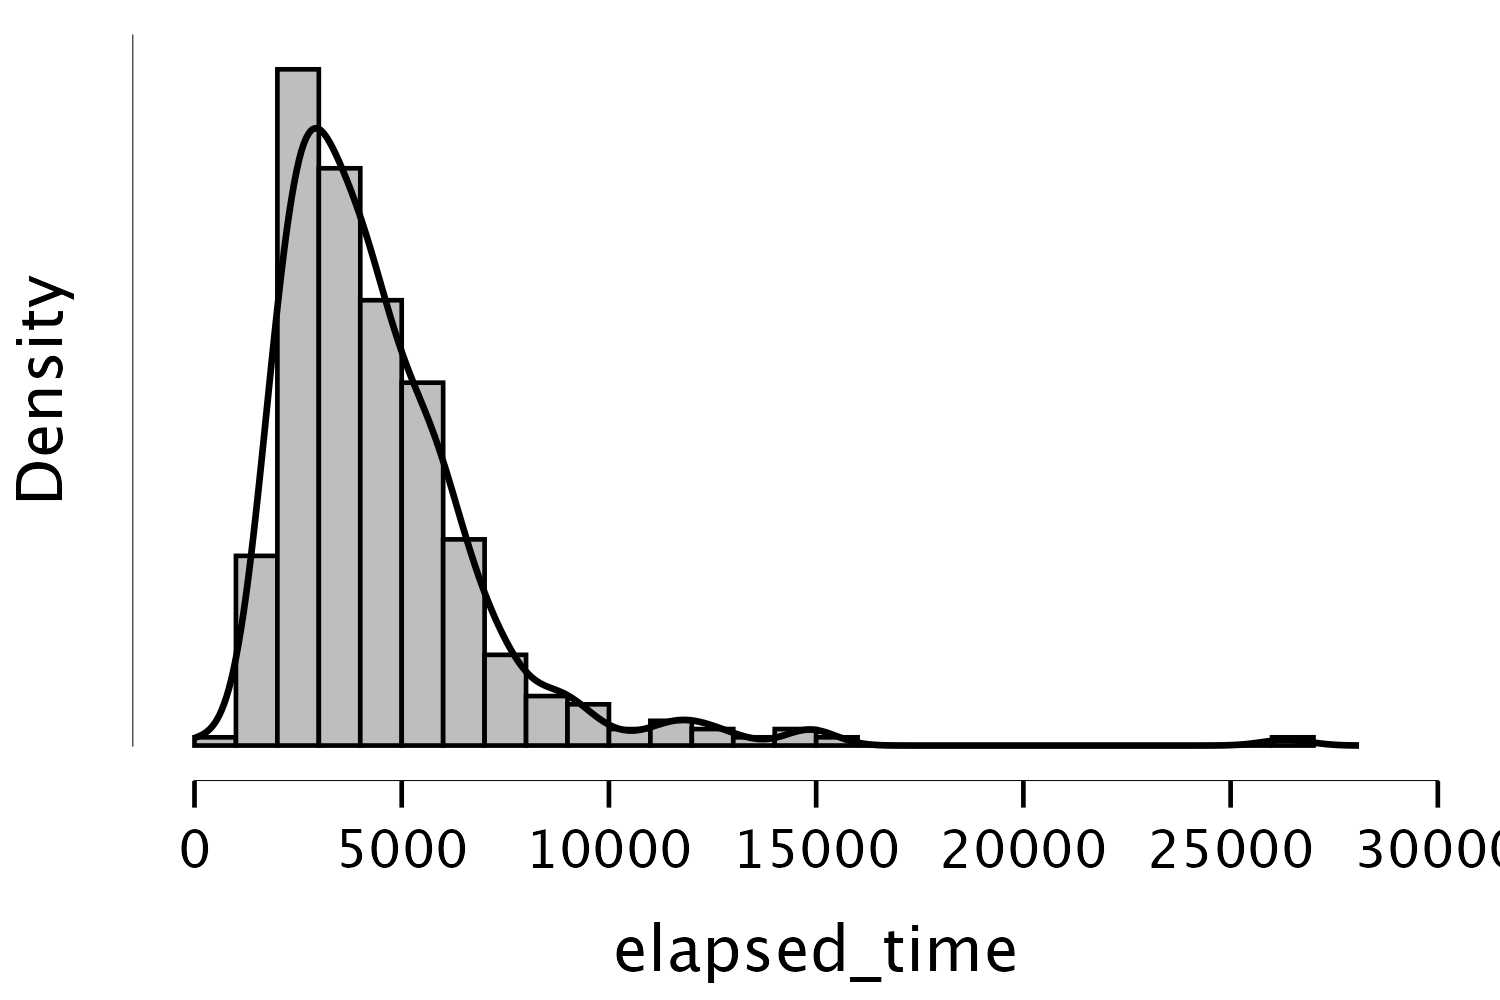
\includegraphics[width=\textwidth]{./figures/correct_camel_distr.png}
        \caption{Distribution of Correct Answers for \texttt{camelCase}}
        \label{fig:correct_camel_distr}
    \end{minipage}
    \hfill
    \begin{minipage}{0.45\textwidth}
        \centering
        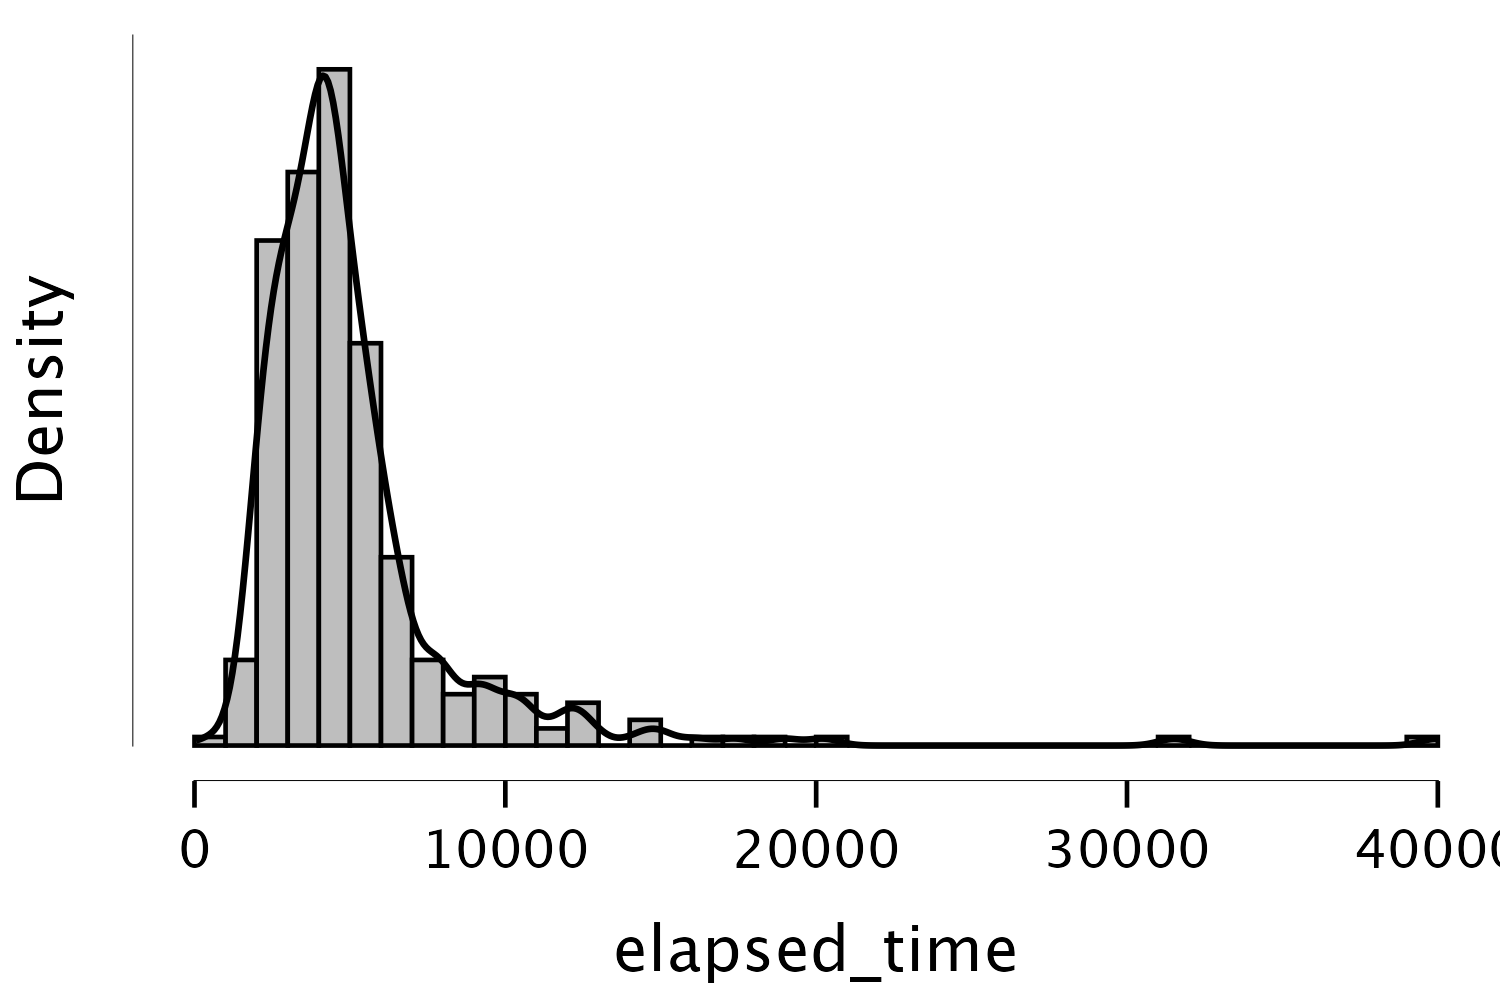
\includegraphics[width=\textwidth]{./figures/correct_kebab_distr.png}
        \caption{Distribution of Correct Answers for \texttt{kebab-case}}
        \label{fig:correct_kebab_distr}
    \end{minipage}
\end{figure}

The distributions in Figure \ref{fig:correct_camel_distr} and Figure \ref{fig:correct_kebab_distr} exhibit a right-skewed shape, where most correct answers occur at a shorter elapsed time. In Figure \ref{fig:correct_camel_distr}, the \texttt{camelCase} distribution peaks slightly earlier, meaning faster response times. Figure \ref{fig:correct_kebab_distr} shows a longer tail, suggesting that some participants took more time to answer. \\
The data shows that \texttt{camelCase} was slightly faster, while the \texttt{kebab-case} times were a bit more spread out, but followed the same basic shape. The long tails may indicate that some identifiers were harder to understand, or that some participants were more familiar with one case style over the other. \\

These observations suggests that \texttt{camelCase} led to faster responses on average and more consistent performance. In contrast, \texttt{kebab-case} resulted in more variation, with some participants taking much longer to respond.

Overall, while both naming conventions were readable, \texttt{camelCase} seems to be on average faster for participants.

\newpage

\subsection{Descriptive Statistics}

\begin{table}[h!]
    \centering
    \caption{Descriptive Statistics of All Participants}
    \label{tab:all}
    \resizebox{\textwidth}{!}{
        \begin{tabular}{rrrrrrrr}
            \toprule
                       & Mean       & Std. Deviation & Minimum   & Maximum     & 25th percentile & 50th percentile & 75th percentile \\
            \cmidrule[0.4pt]{1-8}
            \texttt{camelCase}  & $4442.718$ & $2609.916$     & $150.000$ & $26341.000$ & $2734.000$      & $3904.000$      & $5522.000$      \\
            \texttt{kebab-case} & $5119.937$ & $3691.977$     & $497.000$ & $39951.000$ & $3209.500$      & $4319.000$      & $5624.000$      \\
            \bottomrule
        \end{tabular}
    }
\end{table}

Table \ref{tab:all}, which includes all participants, shows that the average response time for \texttt{camelCase} is 4442 ms, compared to 5119 ms for \texttt{kebab-case}. The smaller standard deviation for \texttt{camelCase} (2609 ms) suggests that responses were more consistent. \\


\begin{table}[h!]
    \centering
    \caption{Descriptive Statistics of Participants with a Programming Background}
    \label{tab:bg}
    {\resizebox{\textwidth}{!}{
            \begin{tabular}{lrrrrrrrr}
                \toprule
                              &            & Mean       & Std. Deviation & Minimum   & Maximum     & 25th percentile & 50th percentile & 75th percentile \\
                \cmidrule[0.4pt]{1-9}
                elapsed\_time & \texttt{camelCase}  & $3969.640$ & $2113.221$     & $150.000$ & $15059.000$ & $2548.250$      & $3511.000$      & $4987.750$      \\
                              & \texttt{kebab-case} & $4567.916$ & $3290.778$     & $328.000$ & $39951.000$ & $3007.250$      & $4007.500$      & $5118.750$      \\
                \bottomrule
            \end{tabular}
        }
    }
\end{table}

In Table \ref{tab:bg}, participants with programming experience appear to respond faster on average. For \texttt{camelCase}, the mean response time is 3969 ms, while \texttt{kebab-case} shows a higher mean of 4567 ms. This may suggest that \texttt{camelCase} could be slightly easier or quicker to process for programmers. The smaller standard deviation for \texttt{camelCase} (2113 ms) compared to \texttt{kebab-case} (3290 ms) indicates more consistent response times, in line with the trends for all participants. 
\\

\begin{table}[h!]
    \centering
    \caption{Descriptive Statistics of Participants without a Programming Background}
    \label{tab:nobg}
    { \resizebox{\textwidth}{!}{
            \begin{tabular}{lrrrrrrrr}
                \toprule
                              &            & Mean       & Std. Deviation & Minimum    & Maximum     & 25th percentile & 50th percentile & 75th percentile \\
                \cmidrule[0.4pt]{1-9}
                elapsed\_time & \texttt{camelCase}  & $5296.818$ & $3376.998$     & $1744.000$ & $26341.000$ & $3200.250$      & $4419.500$      & $6334.250$      \\
                              & \texttt{kebab-case} & $6310.291$ & $4330.106$     & $1771.000$ & $31522.000$ & $3637.000$      & $4952.500$      & $7584.250$      \\
                \bottomrule
            \end{tabular}
        }}
\end{table}

In Table \ref{tab:nobg}, participants without programming experience seem to take longer overall. The average response time for \texttt{camelCase} is 5296 ms, while for \texttt{kebab-case} it is 6310 ms. This could mean that \texttt{camelCase} might be processed more quickly by non-programmers as well. \\

Overall this indicates that \texttt{camelCase} seems to be faster than \texttt{kebab-case}.



\subsection{Inferential Statistics}

\begin{table}[h!]
    \centering
    \caption{Paired Samples T-Test}
    \label{tab:pairedSamplesT-Test}
    {
        \begin{tabular}{lrrrrrrr}
            \toprule
            Measure 1  &   & Measure 2 & t       & df    & p       & Cohen's d & SE Cohen's d                                                             \\
            \cmidrule[0.4pt]{1-8}
            \texttt{kebab-case} & - & \texttt{camelCase} & $3.515$ & $359$ & $1.000$ & $0.185$   & $0.064$                                                                  \\
            \bottomrule
            \addlinespace[1ex]
            \multicolumn{8}{p{0.8\textwidth}}{\textit{Note.} For all tests, the alternative hypothesis specifies that \texttt{kebab-case} is less than \texttt{camelCase}.} \\
        \end{tabular}
    }
\end{table}

Table \ref{tab:pairedSamplesT-Test} shows the results of a paired samples t-test. We compares response times for \texttt{kebab-case} and \texttt{camelCase}. The test revealed that the observed difference in response times was not statistically significant (\textit{t}(359) = 3.515, \textit{p} = 1.000). The small Cohen's \textit{d} value of $0.185$ tells us that even when people were faster with \texttt{camelCase}, the difference is not statistcally relevant.

Even though the descriptive statistics analysis showed that people were generally faster and more consistent with \texttt{camelCase}, these inferential statistic results suggest that this effect is not significant. This outcome supports the null hypothesis that there is no significant difference in reading speed between the two case styles.


\section{Discussion}
\subsection{Comparison of Hypotheses with Results}
The results support the null hypothesis: there was no significant difference between \texttt{kebab-case} and \texttt{camelCase} in terms of response times. Although \texttt{camelCase} appeared slightly faster in descriptive statistics, this difference was not statistically significant.

For participants with programming experience, the mean response time for \texttt{camelCase} was about 600 ms faster than for \texttt{kebab-case}. Non-programmers showed a larger descriptive difference of around 1000 ms, with \texttt{camelCase} being faster. However, the inferential statistics suggest these differences could be due to random variation, as the effect size was small. Furthermore, we observed that non programmers were more accurate than programmers, which could be due to the fact that they took more time to answer.
\subsection{Implications}
While \texttt{camelCase} showed a slight advantage in speed and consistency, the lack of statistical significance means that neither style can be declared superior for reading comprehension tasks. This is consistent with the idea that naming conventions are mainly a matter of preference, familiarity or other factors. 

\subsection{Limitations and Threats to Validity}
This study has several limitations:
\begin{itemize}
    \item The sample size of 36 participants may have been too small to detect subtle differences.
    \item The participants were mainly Informatics students, meaning that the sample was not representative of the general population of programmers.
    \item Variations in participants' familiarity and preferance with naming conventions could have impacted response times.
    \item The experiment doesn't really replicate real-world coding environments, where identifier complexity may differ.
    \item The study does not consider the impact of the participants' native language.
\end{itemize}

\subsection{Conclusion}
The findings indicate that both \texttt{camelCase} and \texttt{kebab-case} are highly readable, with no significant performance difference in terms of speed or accuracy. While \texttt{camelCase} appeared slightly faster and more consistent, this effect was small and not statistically significant. Future research with larger sample sizes and more complex tasks could provide further insights into how naming conventions influence code readability and comprehension.

\section{Appendix}
\subsection{Reproduction Package}

// todo davide aggiungere link
// todo davide scrivere il readme


\end{document}